\chapter{Introduction}
\label{chap:introduction}


\section{Emergence of the Distributed Ledger model}

Ledgers have values as \textit{archives}, or, in other words, their value is their capability of being consulted to check, verify and manage records.

Ledgers have been a central element of commerce since ancient times, and are used to record a variety of informations, ranging from financial assets to real estate properties, but most importantly how these change hands, that is, transactions.

The medium on which transactions have been stored may have changed from clay tablets to hardware storage, but in all this time there haven't been notable innovations to the underlying architecture of the system.
Each financial institution (i.e. banks, governments, investment funds) manages its own ledgers, each designed differently based on necessities, goals and customers (the would-be \textit{counterparts} in the transaction), and in turn, the counterparts keep recorded their own views of the transactions.

This duplication of information amongst all parties partecipating in the transaction drives a need for costly matching between each copy of the information, reconciliation and error fixing. The plurality of technology platforms upon which financial entities rely adds to that, creating more complexity and operational risks, some of which potentially systematic. 

For example, let's consider the need for a party to transfer an asset, be it cash or a stock, to another party. The transaction itself can be executed in microseconds, but the settlement - the ownership transfer of the asset - usually takes more time, from days to weeks.
This length is due to different reasons: the parties don't have access to each other's ledgers, and can't automatically verify that the assets about to be transferred are in fact owned and not counterfeit. So a number of intermediaries are needed as guarantors of the assets and to verify the transaction. 
A number of steps have to be added just for this trusting mechanism, and in addition, the differences between infrastructures and technologies of each party acting in the transaction can be such that there's always a need for reconciliation process between parties (ie adjusting each ledger to the transaction), increasing costs and length of the operations.  

Centralized infrastructures were until recently an unavoidable model, as there were few ways to consolidate technologies without effectively consolidating the financial entities themselves. The industry has been moving toward the standardization and sharing of data and some of the business logic behind the architectures through the delegation of some part of the process to third-parties, but these steps are still lagging behind the evolution of the technology. 

\begin{figure}[t]
    \centering
    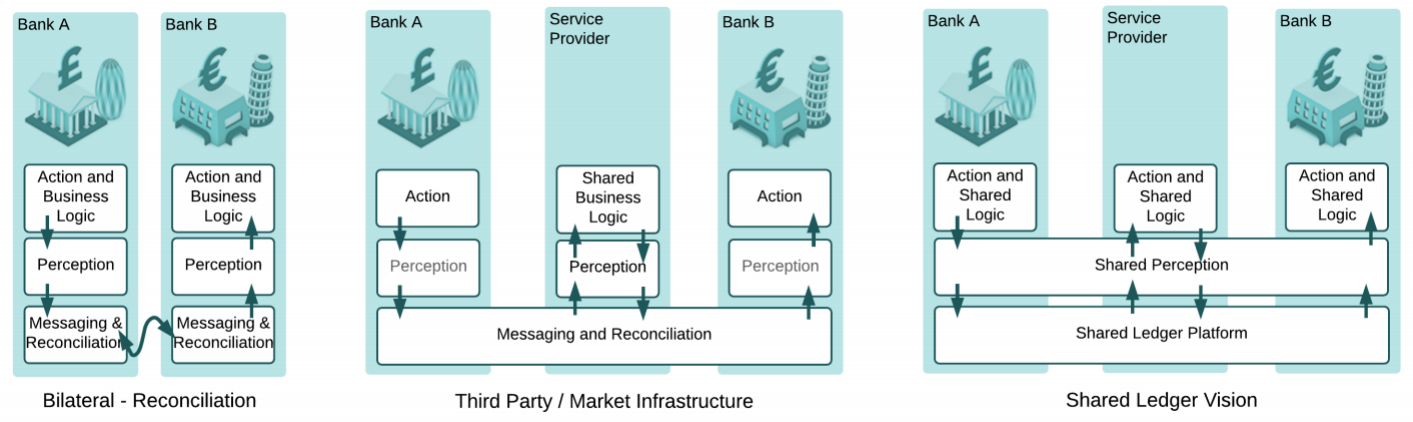
\includegraphics[scale=0.3]{architectures-comparison.png}
    \caption{
        Comparison between architectures, \cite{cordawhitepaper}. 
        }
\end{figure}


The term Distributed Ledger Technology refers to the processes, protocols and technologies that enable nodes in a distributed network to share data (propose, validate and record) between multiple synchronized data stores, collectively maintaned. The emergence of this technologies has had a stimulating effect in the FinTech industry, prompting the reconsideration of the entities needed in a financial transaction, how should trust be established, the representation of the transaction, the securing of data, and many more. Even if DLT is not the answer in every case, asking these questions alone can be a force to drive progress forward.

\section{Brief history}
In 2008, a white paper (\cite{bitcoinpaper}) written by an as yet unidentified person using the pseudonym of Satoshi Nakamoto, outlined a novel approach of transferring cash from one party to another without the need for a known and trusted third-party in a P2P manner, claiming, amongst other things, to have solved the issue of double-spend for digitalized currencies. 


The technology outlined in the paper was named Blockchain, referring to the way of organizing data and transactions. Bitcoin has soared in terms of popularity and value through its cryptocurrency market, but is just one element in its whole architecture. \\

The effort of the industry since the introduction of blockchains has been directed to exploring different ways of leveraging this technology beyond Bitcoin, focusing on the core architecture of distributed record management. This use has gathered significant attention, reflecting the financial industry traditional reliance on multiple ledgers to maintain transactions. The use of DLT would be particularly effective for payment, clearing and settling activities because of the potential for simplification of the settling and reconciliation process between the parties involved. \\

Some of the resulting implementations of DLTs have been on a steady rise, such as Ethereum, that similarly to Bitcoin has seen a steep rise to the value of its cryptocurrency, Ether, and unlike its predecessor, offers a more malleable enviroment (which is the main reason Vitalik Buterin created it), allowing for the transfer and recording of other assets like loans or contracts. Other rising implementations include R3 Corda, which showcases architecture heavily based on financial use-cases, IBM Hyperledger Fabric and Digital Asset Platform.

As the research and development of the technology progresses, real-world applications have highlighted some of the challenges associated with these use-cases, including the need for safe, secure and scalable systems. \\

As of 2018, the impact of DLTs in the financial sector seems still circumvented. Despite strong progress in the research, it would seem that in the near-to-medium term many of the benefits and efficiency gains of DLT are likely to be reaped by start-ups and financial institutions in the developing countries, such as ABRA,\nocite{abracompany} a company that offers instant P2P money transfers with no transaction fees through the Abra Network, combining cryptocurrencies with physical bank tellers; Ripple,\nocite{ripplecompany} that similarly deals in commercial cross-border and inter-bank payments with a peculiar dynamic approach towards transactions, where the flow of funds between a sender and receiver can go through a series of partecipating institutions that offer services (making customers, for example, find better foreign exchange transactions); ShoCard,\nocite{shocardcompany} a digital identity card that stores ID information on the Bitcoin blockchain, with the company currently being in the process of developing solution for different use cases like identity verification, fiancial services credentialing or automated registrations for online purchases. \\


\begin{figure}[h]
    \begin{tcolorbox}[colframe=boxcolor]
        \section*{What is a blockchain?}
        The term blockchain refers to the most well-known configuration of DLTs, and refers to a distributed ledger architecture where the data is stored in entities called transaction blocks, linked with each other through chained encryption. The blockchain itself is the data structure formed by these linked blocks. Blockchains make use of algorithmic methods and encryption to ensure immutability, security and truthfulness of the information.
        
        New additions are initiated by one of the nodes that creates a new block of data, containing the encrypted transactions. Information about the block is then shared on the network, and all participants collectively try to determine the block's validity according to a pre-defined alghoritmic validation method (consensus). After the validation, all the participant can add the block to their copy of the ledger. With this mechanism, every change to the ledger is replicated across the entire network, and each node has a full, identical copy of the entire ledger at any point in time. As the chain grows and new blocks are added, earlier blocks cannot be altered. \\

        The cryptocurrency aspect is what has made Bitcoin garn the most fame. Bitcoin was designed specifically for creating a digital currency free of government control, while also anonymizing the identity of the participants.
        The consensus process involves the generation of a reward to the node that validated the last block of the blockchain, that being the currency in itself. 
    \end{tcolorbox}
\end{figure}

\begin{figure}[h]
    \begin{tcolorbox}[colframe=boxcolor]
        \section*{Double-spending}
        Double-spending is an issue unique to digital currencies, and is the risk that a digital currency can be spent twice. Physical currencies do not have this issue, as they're not easily reproduced, but digital information, on other hand, is easily replicated. \\

        With digital currency, there is a risk that its holder could make a copy of the digital token and send it to another party, while retaining the original. 
        
    \end{tcolorbox}
\end{figure}
\newpage

\section{Distributed Ledger taxonomy}

It is emphasized that DLT is not a single, well-defined technology, but as of today there is a plurality of blockchains and distributed ledgers in active development.

DLs can be designed in a number of ways pertaining to main idea behind them and the use-cases they're designed to respond to. Such arrangements usually involve several key technical design concepts that specify how the information has to be kept on the ledger and how the latter has to be updated. 
There usually are four core attributes of DLTs, these are:
\begin{enumerate}
    \item The distributed nature of the ledger
    \item The cryptographic mechanisms
    \item The consensus mechanism
    \item The network access permission level
\end{enumerate}

These four elements play are fundamental in ensuring the distributed ledger ability to store and exchange data across different, self-interested parties, without the need for a central record-keeper, without the need for trust amongst the concerned parties, as it is guaranteed by the system itself, and while assuring that no double-spending takes place. Each DLT addresses these attributes in their own specific way, but their abstract taxonomic aspects remain the same.

\subsection{Distributed nature of the ledger}
In its simplest form, a distributed ledger is a data store held and updated by each participant (or node) in a network. The control over the ledger does not lie within any single entity, but within several, if not all the network participants. This sets the technology apart from cloud computing or data replication, which are commonly used as shared ledgers.

There are different configurations to be analyzed regarding how the data is maintained over the ledger. 
In blockchains, no single entity of the network can amend past data entries, and no single entity can approve new additions to the ledger, which have to go through a predefined consensus mechanism. At any point in time there exists only one version of the ledger, and each network participant owns a full and up-to-date copy of it.
After validation the new transaction(s) are added to all the ledgers to ensure data consistency across the network.
In configurations like Corda's, each node maintains a separate ledger. The entirety of the ledger is the union of these ledgers, but isn't public, each peer can only see a subset of the facts on the ledger, and no peer is aware of the ledger in its entirety. This is due to Corda's design, where data is shared only on a need-to-know basis and only to directly involved parties.

Generally, this distributed nature of DLs allows the removal of a trusted central party, increasing speed and potentially removing friction costs and inefficiencies associated with the matching and reconiculiation processes. It also improves security, removing the single point of attack and single point of failure that is represented by the central trusted entity. To potentially gain control over the network, a malicious third party would have to gain control over 50\%+1 nodes in the network. 

Security risks aren't completely solved: the software layer built over the distributed ledger can become an additional attack surface.

\subsection{Cryptographic mechanisms}

Cryptography is at the core of the DLT. Asymmetric cryptography plays an important role by identifying and authenticating participants, confirming data entries and facilitating ledger updates.
Each data entry is hashed, producing the so-called digest. The data is in this way hidden to anyone that is not intended to look at it, as the digest, which looks random and unrelated to the original input, is in fact deterministic, meaning that from one original input there's only one hash possible. Digital signatures, which are a common and robust method used in a wide array of application are used as a means of authentication. Each network participant has a private key, that is used for signing digital messages and only known to the key owner, and a public key, which is public knowledge and used for validating the identity of the sender of the original message.
participants proposing changes will authenticate themselves using digital signatures, and the validators will use cryptographic tools to verify whether the participant has the proper credentials, and so on. The validators can be either a counterpart, a third party, or the whole network depending on the type of DL and operation the change refers to.

In the blockchain subset of DLs in particular, encryption plays a fundamental role, as they're essential in the chain encryption mechanism between the blocks that make up the blockchain itself.


\subsection{Consensus mechanism}
\label{sec:consensus}
The purpose of the consensus mechanism is to verify that the information being added to the DL is legitimate. It is fundamental in handling conflicts between multiple simultaneous competing entries (ie double spending), or take-overs by bad actors in the network. It's a derivative property of the distributed nature of the ledger, and it requires participants in the network to reach a consensus over the information being added. There exist many different consensus algorithms and mechanisms, with different purposes, advantages and disadvantages. \\

Consensus usually involves two steps:
\begin{enumerate}
    \item Validation, where each validator involved identifies that the state change is consistent according to the rules of the ledger. This operation may rely on records of previous states or a last agreed state.
    \item Agreement, where each validator agrees to the state changes to the ledger. This step involves the mechanisms to resolve eventual conflicts and ensuring that valid changes are made only once, thus ensuring that the whole network is synchronized.
\end{enumerate}

According to the DLT configuration, the mechanisms to avoid double-spendings fit in either of the two steps. \\

The Bitcoin blockchain uses Proof-of-Work (PoF) to establish consensus. To add a new block to the blockchain, a node has to provide a proof of work. This is a computationally taxing problem, but easy to verify, and is solved by brute-forcing cyptographic hashing algorithms until the correct string that satisfies certain conditions is generated. This process is called "mining". Each miner that produces a valid PoF is then rewarded Bitcoins, which serves as an economic incentive to maintain system operation and integrity.\\

The Ethereum blockchain uses Proof-of-Stake (PoF). Its process is quite different from the PoF of Bitcoin, as there's no mathematical problem to solve, but instead, the creator of the new block is chosen in a deterministic way based on their stake, that is, how many coins or tokens they possess. 
A key advantage to this approach is the energy efficiency. The Bitcoin network, for example, requires an annual energy consumption comparable to that of Columbia (57.6 TWh annually). 
Thus PoS systems are well suited to platforms where there is a static coin supply, without inflation from block rewards. The rewards consist only in the transaction fees. \\

\begin{figure}[h]
    \centering
    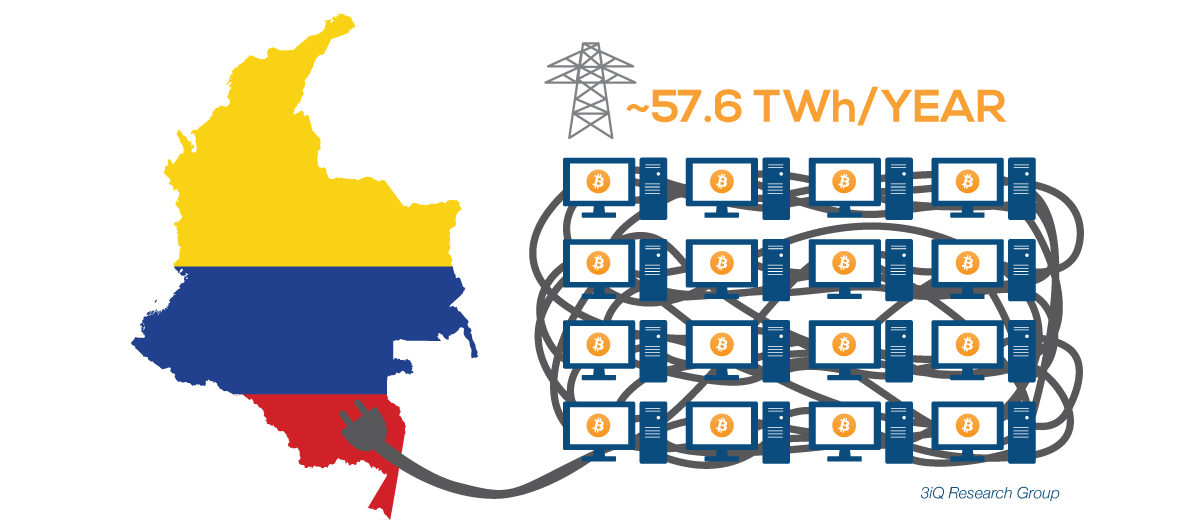
\includegraphics[scale=0.3]{bitcoin-energy.png}
    \caption{
        Data as at April 3rd, 2018. Retrieved from https://digiconomist.net/bitcoin-energy-consumption}
\end{figure}

The Corda distributed ledger, utilizes a unique "pluggable" consensus service, due to its peculiar distributed ledger architecture. It divides consensus in two types, validity consensus and uniqueness consensus. Given a proposed transaction, the first type of consensus checks whether the two parties satisfy a set of validity conditions, going back through all the parties' transaction histories, while the latter has the purpose to avoid double spend, and the consensus is provided by a Corda network service called "Notary", by attesting that, for a given transaction, there hasn't been proposed another competing one.\\


\subsection{Network access permission level}

The partecipation in the DL network can be open (permissionless) or permissioned. Bitcoin and Ethereum are the most prominent examples of completely permissionless blockchain, where participants can join or leave the network at will. This plays as one of their strengths, as a large, open permissionless system with a large number of nodes incentivized to validate new changes to the ledger and accurately and establishing a consensus is directly related to its network security (\ref{sec:consensus}).

In permissioned DLs its members are pre-selected by someone - an owner, or a network service - who controls network access and sets the rules of the ledger. The regulations of network access usually permit the use of a non-computationally expensive consensus mechanism, as there is no need for any trust between participants. This, however, means there's now a centralized trust entity playing a coordinating role and bearing the responsibility over the trusting mechanism. 
In permissioned DLs it's possible to have different degrees of transparency over the ledger, and faster transaction processing (thanks to the lighter consensus algorithm) allows for higher transaction volumes.

The identity verification needed for the access solves some problems with governments and regulators with concerns about the identity verification and legal ownerships clarifications. \\

Permissionless DLs have open access to the network, so anyone can join and leave as they wish. There's no central owner or administrator, the ledger is wholly transparent and the security is established by having a large scale network. It is required to have a complex consensus algorithm to guarantee the integrity of the information, and there are some legal concerns over the lack of ownership, as no legal entity owns or controls the ledger.

Some industry players make distinctions between public/private, in term of access, and permissioned/permissionless, in term of roles in the network. For example, Ripple has a permissioned ledger, but the data is validated by all participants, therefore being a public, permissioned ledger. Corda, on the other hand, has a permissioned ledger, but the data is validated only by a set of participants (those which the data concerns), hence being a private, permissioned ledger.

\begin{figure}[h]
    \centering
    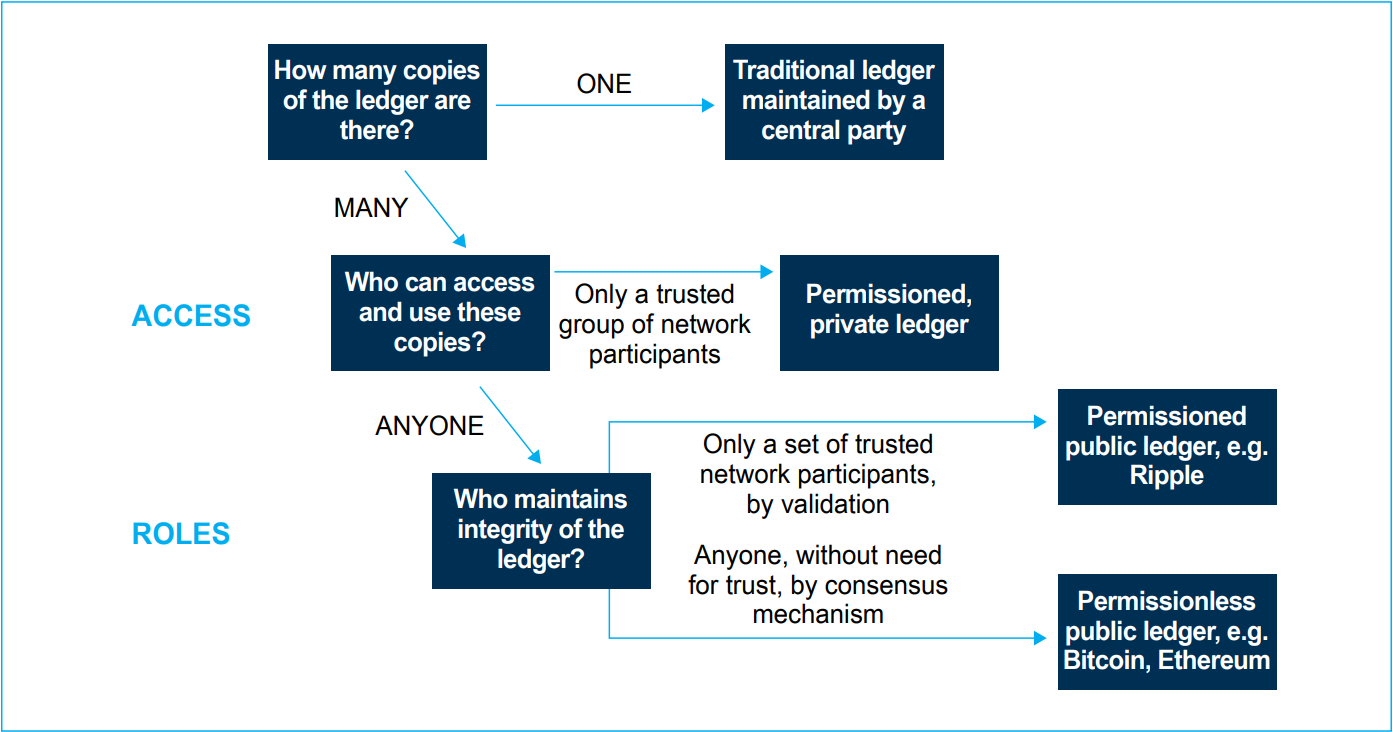
\includegraphics[scale=0.3]{permissioned-permissionless-taxonomy.png}
    \caption{
        Network Access Ledger Taxonomy, \cite{ukgovdltpaper}. 
        }
\end{figure}

\begin{figure}[b]
    \begin{tcolorbox}[colframe=boxcolor]
        \section*{What are smart contracts?}
            Smart contracts are self-executing contracts with the terms of the agreement between two parties of a transactions, written as code. The code and the agreement exist distributed across a distributed ledger network. Smart contracts allow for trusted transactions and settlements to be carried out among different and possibly anonymous parties without the need for a central authority, legal system or enforcement mechanism. They render transaction transparent, irreversible and traceable. 
    \end{tcolorbox}
\end{figure}

\subsection{Roles}
Nodes in the network may play a variety of roles, depending on the participants intentions or technical arrangement of the DL. The Committee on Payment and Market Infrastructures of the Bank for Internation Settlements proposed a generalized framework, with the following different, non-exclusive roles for a node:

\begin{enumerate}
    \item System Administrator: node controlling access to the system and provides dispute resolution and notary services. This role is not required in permissionless DLs.
    \item Asset Issuer: node enabled to issue assets. In the Bitcoin blockchain, there's no entity playing this role as the system creates assets (Bitcoins) by itself, according to its rules.
    \item Proposer: node enabled to propose ledger updates.
    \item Auditor: node enabled to view the ledger, but not to make updates. Can be used by regulators or supervisors.
    \item Validator: node enabled to validate requests for addition of transactions in the ledger. This role is performed by the consensus mechanism in permissionless DLs.
\end{enumerate}


